\subsection{Thiết kế sơ đồ lớp} \label{sec:class_diagram}

Trong kiến trúc microservice, biểu đồ lớp tập trung thể hiện tư duy phân tách module và cấu trúc phần mềm. Để làm nổi bật luồng nghiệp vụ cốt lõi, các phương thức phụ trợ (getter, setter...) đã được nhóm chủ ý lược giản.

Đồng thời, nội dung báo cáo chính chỉ tập trung đặc tả chuyên sâu biểu đồ lớp của các thành phần nền tảng và nghiệp vụ trọng yếu, bao gồm thư viện core, orchestration-service, order-service và ai-service. Biểu đồ lớp của các dịch vụ mang tính chất nghiệp vụ và lưu trữ thông thường như user, admin, cart và product sẽ được chuyển vào phần phụ lục nhằm tối ưu hóa dung lượng và duy trì sự tập trung cho tài liệu thiết kế.

Do giới hạn kích thước hiển thị trong tài liệu, phiên bản đầy đủ với độ phân giải cao được cung cấp tại \href{https://drive.google.com/drive/folders/1bg3YoloCTyKwa6vXfV9YgwM5WIQV_Zcn?usp=sharing}{liên kết đính kèm} nhằm hỗ trợ việc quan sát các thành phần và mối quan hệ giữa các lớp.

\subsubsection{Sơ đồ lớp cho thư viện Core} \label{subsec:core_class_diagram}
Trong quá trình phát triển hệ thống e-commerce với nhiều dịch vụ độc lập, việc quản lý các thành phần chia sẻ đóng vai trò then chốt nhằm duy trì tính nhất quán, đồng thời giảm thiểu tối đa sự dư thừa mã nguồn theo nguyên tắc DRY - Don't Repeat Yourself. Thư viện ecom.core được xây dựng và cấu hình như một module hạ tầng dùng chung cho toàn bộ các dịch vụ Java trong hệ thống. Việc đóng gói hạ tầng vào core không chỉ đẩy nhanh tốc độ phát triển các module mới mà còn tạo ra một kiến trúc vững chắc, dễ dàng bảo trì và mở rộng.

Cấu trúc chi tiết của thư viện này được minh họa trong Hình \ref{fig:core_class_diagram}. Biểu đồ tập trung đặc tả ba nhóm thành phần trọng yếu nhất, bao gồm:

\begin{itemize}
    \item \texttt{base\_dto}: Chuẩn hóa giao tiếp API. Sử dụng Generic Type (<T>) trong BaseResponse và PaginationBaseResponse để tạo bộ khung phản hồi linh hoạt. Lớp BasePaginationRequest đóng gói tham số phân trang, hỗ trợ tích hợp liền mạch với Spring Data JPA.
    
    \item \texttt{eventbus}: Cung cấp VertXBus -- một lớp bao bọc tùy chỉnh cho io.vertx.core.eventbus.EventBus. Lớp này giúp che giấu độ phức tạp và chuẩn hóa luồng giao tiếp hướng sự kiện nội bộ một cách an toàn trong Spring Boot.
    
    \item \texttt{util}: Tập trung logic bảo mật. JwtUtil quản lý toàn bộ vòng đời JWT, kết hợp cùng JwtAuthenticationFilter tích hợp trực tiếp vào Spring Security, đảm bảo đồng bộ cơ chế xác thực và phân quyền trên mọi vi dịch vụ.
\end{itemize}

Bên cạnh ba nhóm thành phần chủ chốt nêu trên, thư viện ecom.core còn quản lý các đối tượng truyền tải dữ liệu phụ trợ, các lớp cấu hình, công cụ ánh xạ dữ liệu, và đặc biệt là tập hợp các sự kiện phân tán phục vụ cho quá trình giao tiếp liên dịch vụ qua Kafka. Tuy nhiên, nhằm đảm bảo tính trực quan và tránh hiện tượng quá tải thông tin cho biểu đồ, các thành phần này đã được chủ ý lược giản khỏi Hình \ref{fig:core_class_diagram}.

\begin{figure}[H]
    \centering
    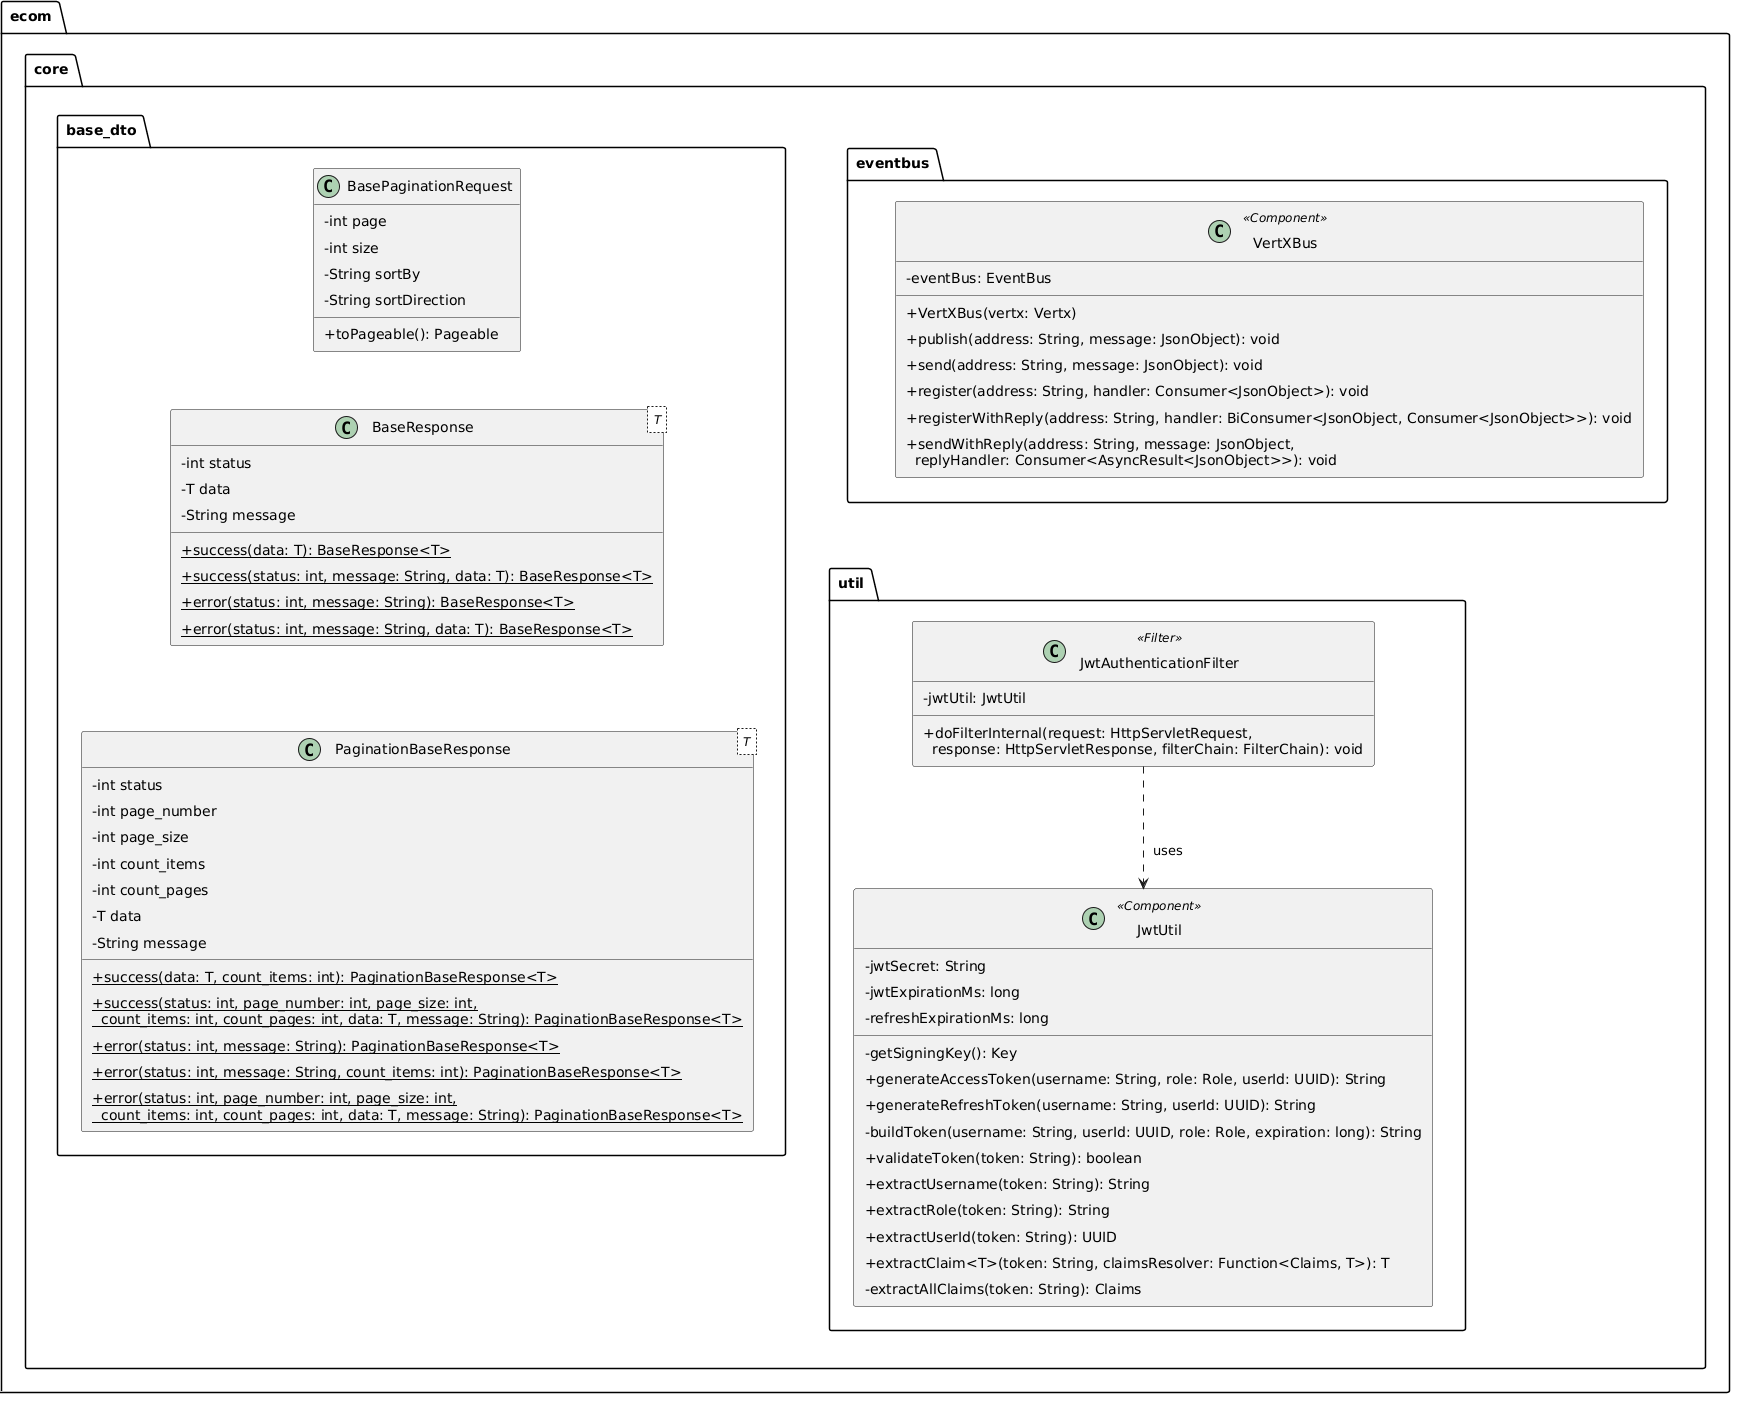
\includegraphics[width=1\textwidth]{images/chap6/class_diagram/core}
    \vspace{0.7cm}
    \caption{Biểu đồ lớp chi tiết của thư viện dùng chung ecom.core}
    \label{fig:core_class_diagram}
\end{figure}

\subsubsection{Sơ đồ lớp cho Orchestration Service} \label{subsec:orchestration_class_diagram}

Hệ thống xây dựng orchestration-service như một tầng điều phối trung tâm dựa trên mô hình Saga kết hợp với Event-Driven Architecture. Nhằm đảm bảo tính trực quan, Hình \ref{fig:orchestration_class_diagram} chỉ tập trung mô tả chi tiết chức năng checkout; các chức năng khác như thanh toán, hủy đơn hàng và các quy trình điều phối khác không được trình bày trong biểu đồ. 

Cấu trúc chi tiết của thành phần được minh họa trong Hình \ref{fig:orchestration_class_diagram}. Biểu đồ tập trung mô tả năm nhóm thành phần trọng yếu bao gồm:

\begin{itemize}

\item \texttt{queries}: Chịu trách nhiệm xử lý các tác vụ truy vấn và tính toán dữ liệu phục vụ giao diện checkout. Lớp dịch vụ này thực hiện tổng hợp dữ liệu từ nhiều nguồn khác nhau như sản phẩm, giỏ hàng, thông tin giao hàng và phương thức thanh toán nhằm xây dựng phiên bản xem trước của đơn hàng.

\item \texttt{command}: Quản lý các thao tác làm thay đổi trạng thái hệ thống. Thành phần CheckoutSagaService đóng vai trò trung tâm điều phối Saga. Dịch vụ này quản lý luồng nghiệp vụ phân tán thông qua các bước xử lý như tạo đơn hàng, đặt giữ sản phẩm và xóa dữ liệu giỏ hàng. Các lớp KafkaConsumer tiếp nhận sự kiện từ các dịch vụ khác nhằm cập nhật trạng thái tương ứng của từng bước trong quy trình.

\item \texttt{client\_interface}: Cung cấp lớp giao tiếp giữa orchestration-service và các dịch vụ bên ngoài thông qua cơ chế FeignClient. Các thành phần như OrderClient, CartClient, UserClient và ProductClient thực hiện truy xuất dữ liệu từ các dịch vụ chuyên biệt, đồng thời đảm bảo tính nhất quán và đồng bộ thông tin trong suốt quá trình checkout.

\item \texttt{repository}: Quản lý thao tác lưu trữ dữ liệu theo hướng tách biệt giữa đọc và ghi. 

\item \texttt{model}: Biểu diễn các thực thể nghiệp vụ cốt lõi của tiến trình checkout. CheckoutSession lưu trữ thông tin phiên thanh toán bao gồm chi phí vận chuyển, giảm giá và tổng giá trị đơn hàng. SagaInstance và SagaStep theo dõi trạng thái từng bước trong quy trình Saga, trong khi OutboxEvent hỗ trợ triển khai mẫu thiết kế Transactional Outbox nhằm đảm bảo tính nhất quán dữ liệu giữa cơ sở dữ liệu và hệ thống Kafka.

\end{itemize}

Kiến trúc của orchestration-service thể hiện việc hiện thực nhất quán các nguyên tắc thiết kế microservice thông qua việc kết hợp Saga Pattern, CQRS và Transactional Outbox nhằm giảm mức độ phụ thuộc giữa các dịch vụ và đảm bảo tính nhất quán cuối cùng của hệ thống.

\begin{figure}[H]
    \centering
    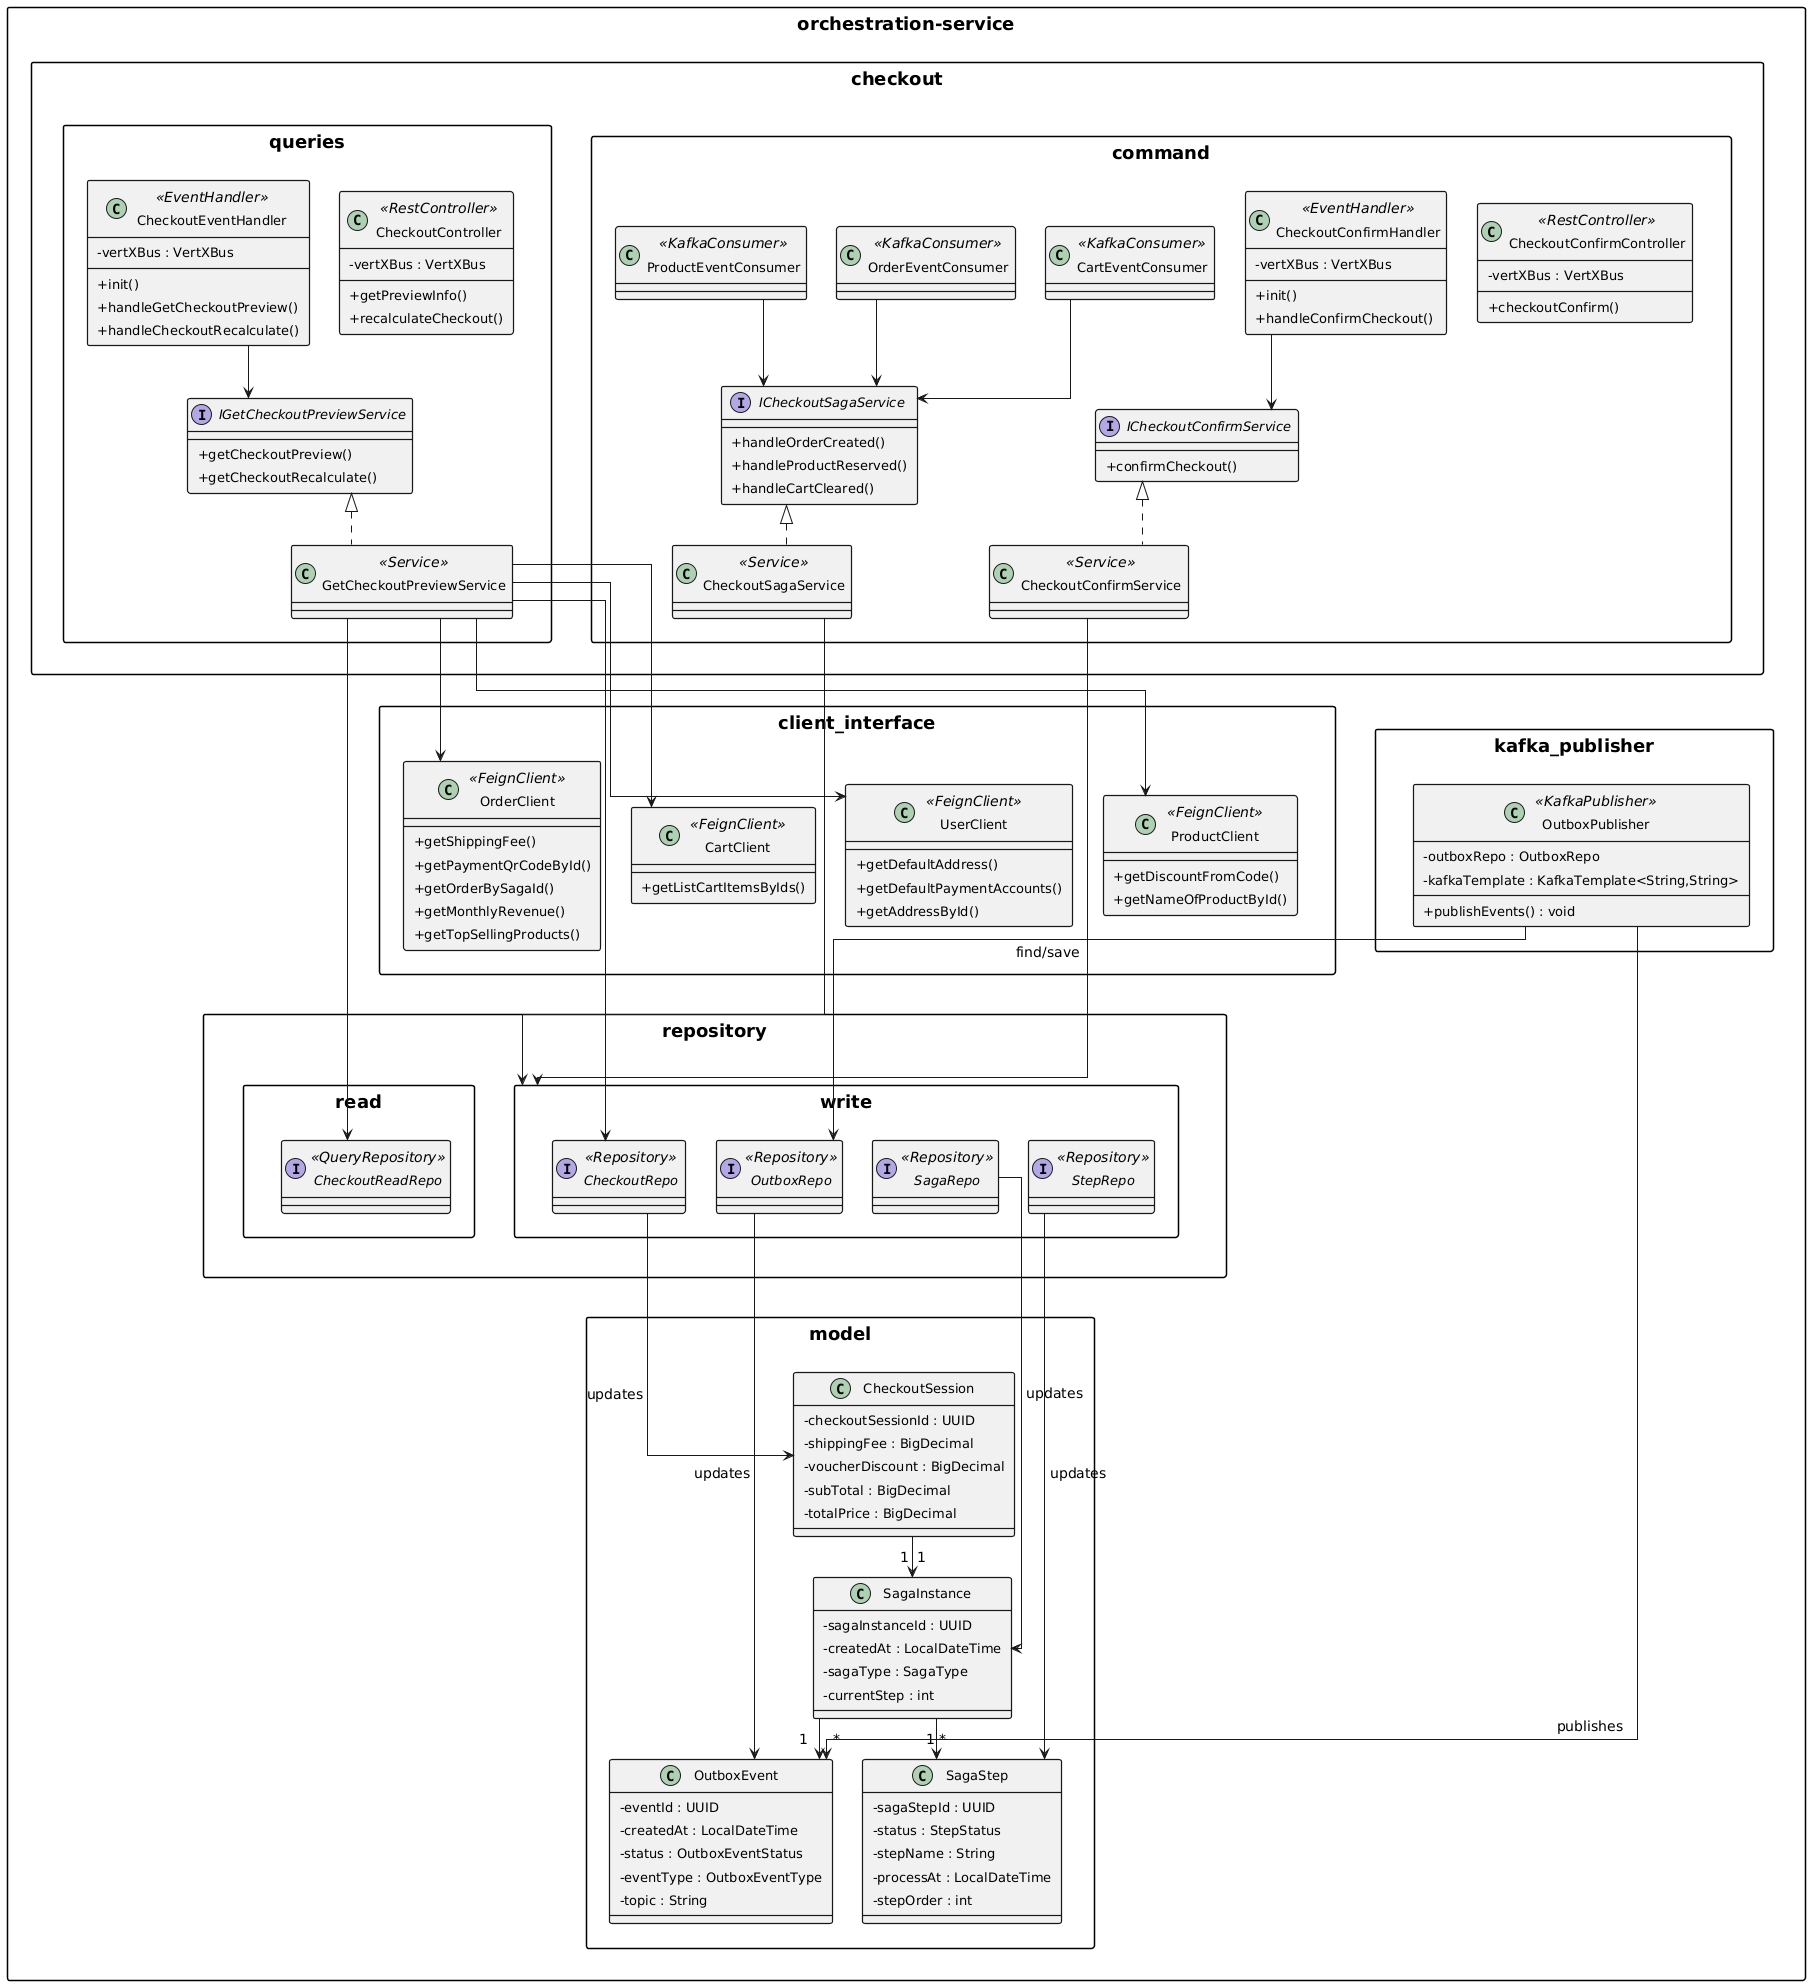
\includegraphics[width=1\textwidth]{images/chap6/class_diagram/orchestration-service}
    \vspace{0.7cm}
    \caption{Biểu đồ lớp chi tiết của orchestration-service}
    \label{fig:orchestration_class_diagram}
\end{figure}


\subsubsection{Sơ đồ lớp cho Order Service} \label{subsec:order_class_diagram}

Trong hệ thống e-commerce, order-service đóng vai trò tiếp nhận, lưu trữ và theo dõi trạng thái của các đơn hàng phát sinh trong quá trình mua sắm. Ngoài việc xử lý vòng đời đơn hàng, dịch vụ còn phối hợp với các thành phần liên quan như thanh toán, đánh giá sản phẩm và vận chuyển nhằm đảm bảo tính nhất quán cho toàn bộ quy trình nghiệp vụ. Tương tự orchestration-service, order-service được xây dựng theo hướng phân tách giữa truy vấn và xử lý trạng thái, kết hợp với cơ chế giao tiếp hướng sự kiện nhằm tăng khả năng mở rộng và giảm mức độ phụ thuộc giữa các dịch vụ.

\begin{figure}[H]\centering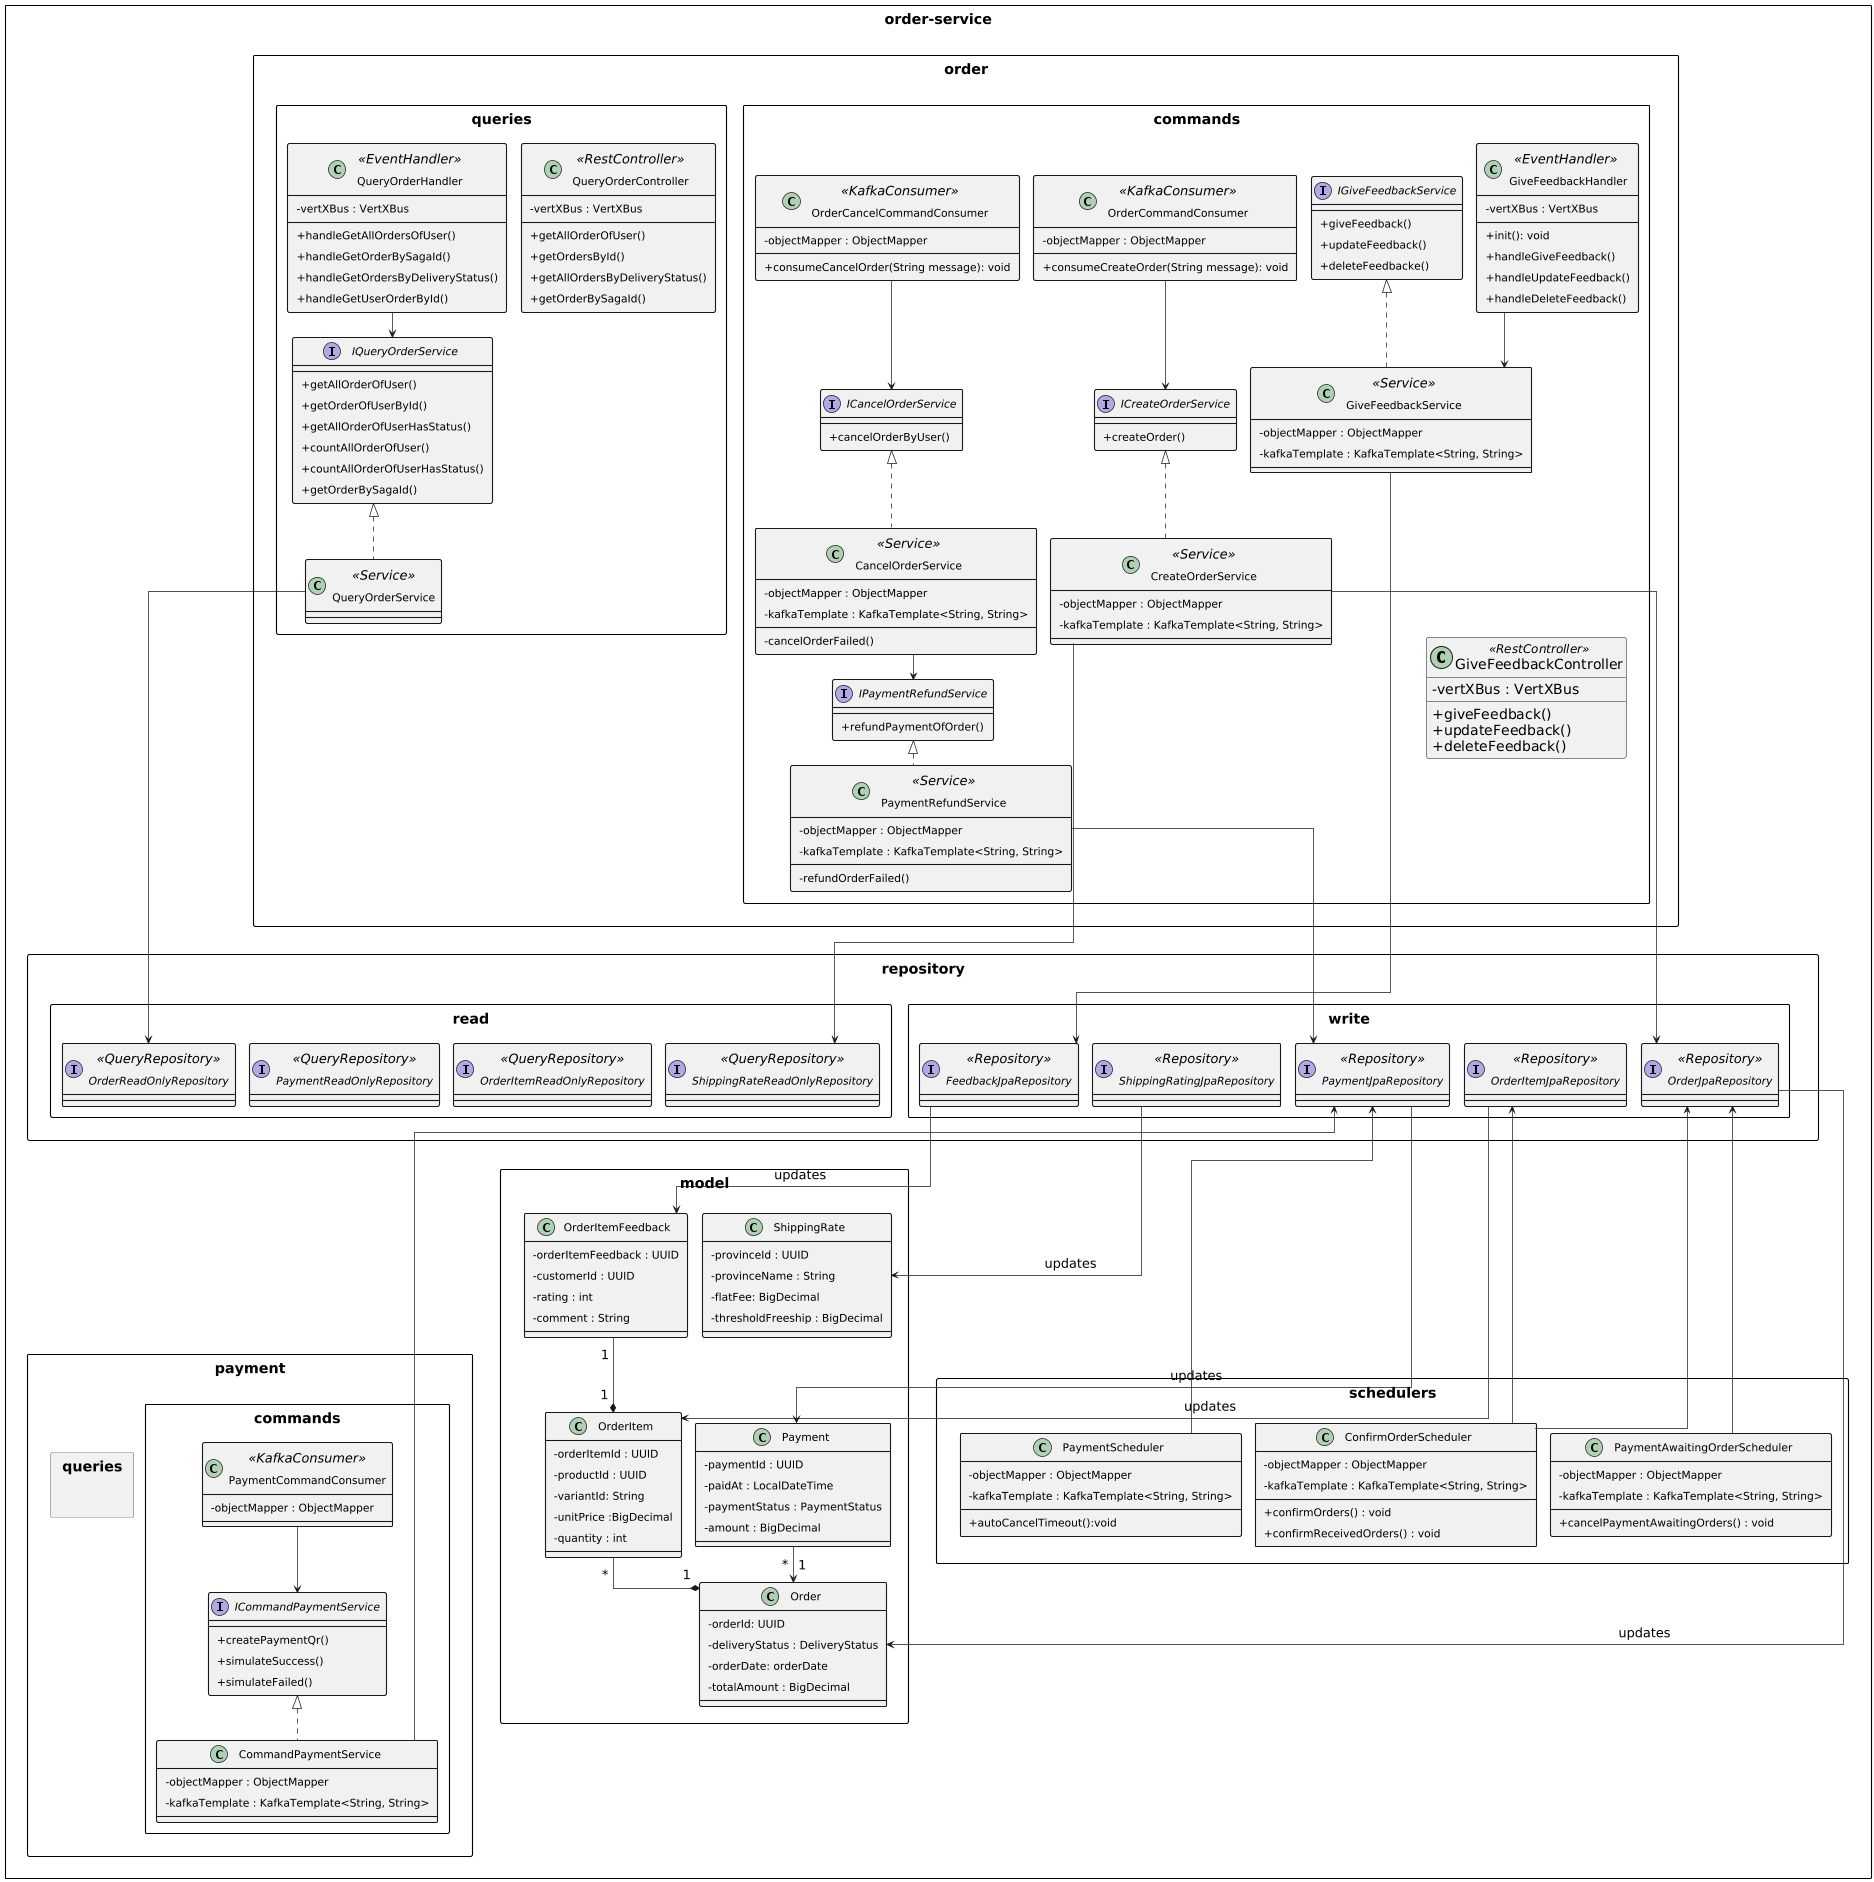
\includegraphics[width=1\textwidth]{images/chap6/class_diagram/order-service}\vspace{0.7cm}\caption{Biểu đồ lớp chi tiết của order-service}\label{fig:order_class_diagram}\end{figure}

Cấu trúc chi tiết của thành phần được minh họa trong Hình \ref{fig:order_class_diagram}. Biểu đồ tập trung đặc tả năm nhóm thành phần trọng yếu bao gồm:

\begin{itemize}

\item \texttt{queries}: Chịu trách nhiệm xử lý các tác vụ truy xuất dữ liệu đơn hàng. Thành phần QueryOrderController tiếp nhận yêu cầu từ phía người dùng, sau đó chuyển tiếp tới QueryOrderService nhằm thực hiện truy vấn danh sách đơn hàng, lịch sử giao dịch hoặc trạng thái đơn hàng theo nhiều tiêu chí khác nhau.

\item \texttt{commands}: Quản lý các thao tác làm thay đổi trạng thái hệ thống. Các thành phần CreateOrderService, CancelOrderService và PaymentRefundService xử lý các nghiệp vụ tạo đơn hàng, hủy đơn hàng và hoàn tiền. Các KafkaConsumer tiếp nhận sự kiện từ các dịch vụ khác nhằm đồng bộ trạng thái đơn hàng trong hệ thống.

\item \texttt{repository}: Quản lý thao tác lưu trữ dữ liệu của hệ thống. Các lớp Repository đảm nhiệm quản lý dữ liệu liên quan đến đơn hàng, thanh toán, đánh giá và chi phí vận chuyển, đồng thời hỗ trợ tối ưu hóa quá trình truy xuất dữ liệu.

\item \texttt{model}: Biểu diễn các thực thể nghiệp vụ cốt lõi của hệ thống. Các lớp Order, OrderItem và Payment lưu trữ thông tin đơn hàng, chi tiết sản phẩm và giao dịch thanh toán; trong khi ShippingRate và OrderItemFeedback quản lý dữ liệu vận chuyển và đánh giá sản phẩm.

\item \texttt{schedulers}: Quản lý các tác vụ nền thực thi theo lịch định kỳ. Các thành phần Scheduler hỗ trợ tự động cập nhật trạng thái đơn hàng hoặc xử lý các đơn hàng chờ vượt quá thời gian quy định.

\end{itemize}

\subsubsection{Sơ đồ lớp cho AI Service} \label{subsec:ai_class_diagram}

Trong hệ thống e-commerce, AI service được xây dựng nhằm hỗ trợ xử lý các tác vụ liên quan đến phân tích dữ liệu và tương tác thông minh với người dùng. Dịch vụ này tiếp nhận dữ liệu từ nhiều nguồn khác nhau trong hệ thống, kết hợp với mô hình tác tử nhằm hỗ trợ gợi ý sản phẩm và xử lý ngữ cảnh hội thoại. 

Cấu trúc chi tiết của thành phần được minh họa trong Hình \ref{fig:ai_class_diagram}. Biểu đồ tập trung đặc tả ba nhóm thành phần trọng yếu bao gồm:

\begin{itemize}

\item \texttt{consumers}: Chịu trách nhiệm tiếp nhận và xử lý các sự kiện phát sinh từ hệ thống thông qua Kafka. Thành phần KafkaWorker và EventHandler thực hiện đồng bộ dữ liệu sản phẩm, thông tin tồn kho, đánh giá và lịch sử mua hàng nhằm duy trì dữ liệu đầu vào phục vụ cho quá trình xử lý của tác tử AI.

\item \texttt{agent}: Là thành phần xử lý nghiệp vụ cốt lõi của hệ thống AI. AgentGraph quản lý luồng thực thi của tác tử, trong khi các thành phần ResolveProducts, Parse và Reason thực hiện phân tích yêu cầu người dùng, suy luận ngữ cảnh và ánh xạ dữ liệu sản phẩm phù hợp. Các lớp AgentState, ResolvedProduct và SpecState lưu trữ trạng thái trung gian phục vụ quá trình xử lý.

\item \texttt{app}: Cung cấp lớp giao tiếp giữa người dùng và hệ thống thông qua AppController và SessionManager. Thành phần này quản lý phiên làm việc, lưu trữ trạng thái hội thoại và xử lý các yêu cầu tương tác từ phía người dùng.

\end{itemize}

\begin{figure}[H]
\centering
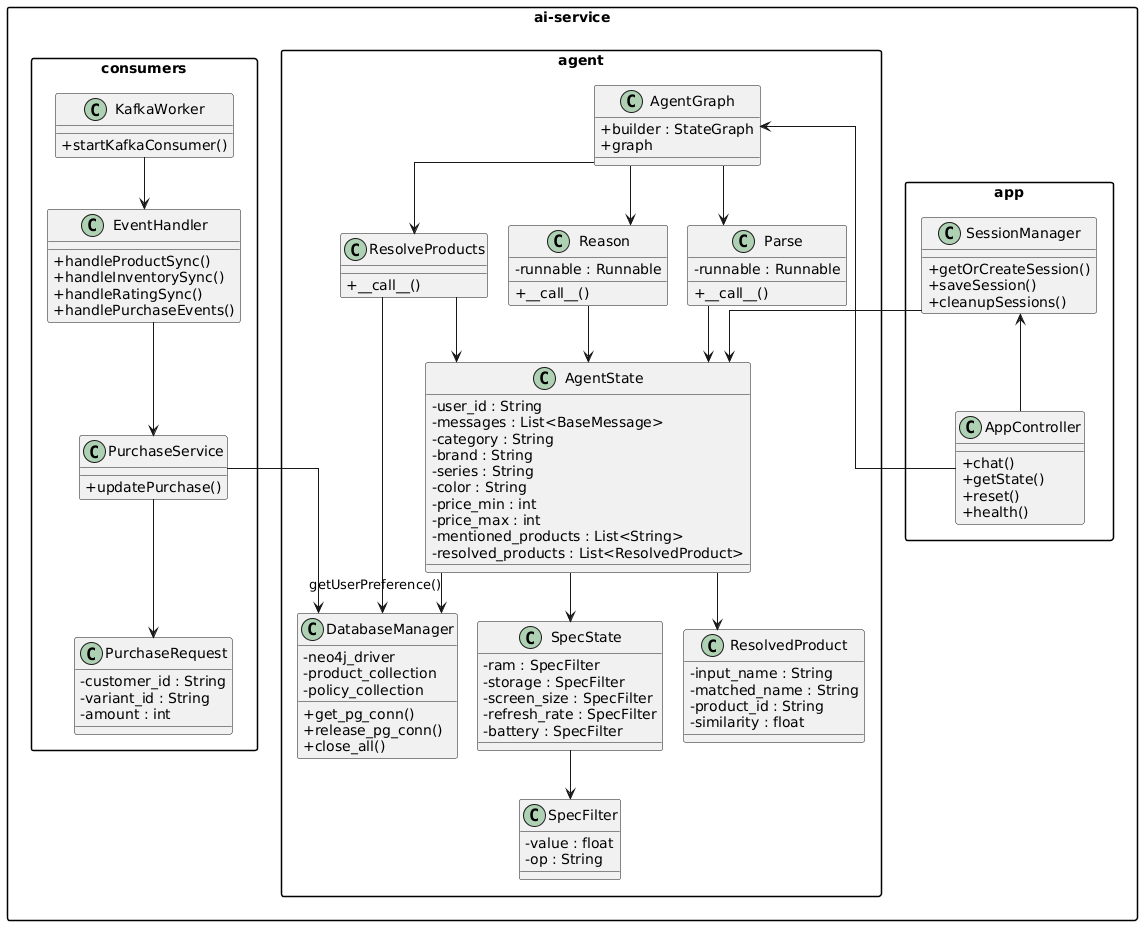
\includegraphics[width=1\textwidth]{images/chap6/class_diagram/ai-service}
\vspace{0.7cm}
\caption{Biểu đồ lớp chi tiết của ai-service}
\label{fig:ai_class_diagram}
\end{figure}

